\documentclass{article}

\usepackage{listings}
\usepackage{makecell}
\usepackage{xcolor}
\usepackage{xurl}
\usepackage{pgf-pie}
\usepackage{pgfplots}
\pgfplotsset{compat=1.8}
\usepgfplotslibrary{statistics}

\renewcommand\theadfont{\bfseries}

% color definition (used for listings)
\definecolor{codegreen}{rgb}{0,0.6,0}
\definecolor{codegray}{rgb}{0.5,0.5,0.5}
\definecolor{codepurple}{rgb}{0.58,0,0.82}
\definecolor{backcolour}{rgb}{0.95,0.95,0.92}

% Designing our listing (Credits to Mutestock : https://github.com/Mutestock)
% He made this style and reviewed an ealier assignment and pointed out that 
% my listing could be improved.
\lstdefinestyle{mystyle}{
    backgroundcolor=\color{backcolour},   
    commentstyle=\color{codegreen},
    keywordstyle=\color{magenta},
    numberstyle=\tiny\color{codegray},
    stringstyle=\color{codepurple},
    basicstyle=\ttfamily\footnotesize,
    breakatwhitespace=false,         
    breaklines=true,                 
    captionpos=b,                    
    keepspaces=true,                 
    numbers=left,                    
    numbersep=5pt,                  
    showspaces=false,                
    showstringspaces=false,
    showtabs=false,                  
    tabsize=2
}

% setting the style to my listings
\lstset{style=mystyle, language=Java}

\author{Anders Jacobsen, Dima Karaush}
\title{Optimization of Letter Frequencies - Take Two}

\begin{document}

\maketitle

\newpage

\tableofcontents

\newpage

\section{Introduction}
We are using the project Letter Frequencies downloaded 
from \url{https://github.com/CPHBusinessSoftUFO/letterfrequencies} 
in this paper. The entire project with all files can be found here 
\url{https://github.com/Cosby1992/CPH-business-assingments/tree/master/Data%20Science/Assignment_3_optimization}.
\newline We plan on measuring a benchmark on the original letter frequencies project. 
This will enable us to see witch aspects of the program is occupying the most runtime.
We plan to use a number of warmup cycles, then run the code again, many times, save the results 
and in the end write it to a csv file for data exploration and visualization. 
We will measure all aspects of the original code, and we plan on splitting the code into 
three categories.
\begin{enumerate}
    \item The initialization
    \item The Letter frequency algoritm
    \item The output to console
\end{enumerate}
We expect to see the letter frequency algorithm to be the bottleneck in this
code. That is because it is at this point in the code we read and handle the reading of the file.
We think that we are able to improve the output to console aswell but not as much as the algoritm. 
We do not have a prediction for the initialization, we expect it to run too fast to have an 
infuence on the execution time, but, we are interested in weather our optimized solution will have
a difference in the initialization execution time.

\section{Test Enviroment}
\subsection{PC and operating system}
\begin{tabular}{ |l|l| }
    \hline
    \thead[l]{OS}                      & Microsoft Windows 10 Pro \\ 
    \hline
    \thead[l]{OS Version}              & 10.0.19042 N/A Build 19042 \\  
    \hline
    \thead[l]{System Type}             & x64-based PC \\
    \hline
    \thead[l]{Processor(s)}            & \makecell[l]{Intel® Core™ i7-10700KF Processor, \\ 16M Cache, up to 5.10 GHz} \\
    \hline
    \thead[l]{BIOS Version}            & American Megatrends Inc. 1.10, 21-05-2020 \\
    \hline
    \thead[l]{Total Physical Memory}   & 32.688 MB \\ 
    \hline
    \thead[l]{Disc(s)}                 & \makecell[l]{Force Series™ MP510 980GB M.2 SSD \\ (up to 3480MB/sec sequencial read)} \\
    \hline
    \end{tabular}
\subsection{Software Enviroment}
\begin{tabular}{ |l|l| }
    \hline
    \thead[l]{IDE}                    & Visual Studio Code \\ 
    \hline
    \thead[l]{IDE version}            & 1.55.2 x64 \\  
    \hline
    \thead[l]{Language}               & Java \\
    \hline
    \thead[l]{Language Version}       & 15 \\
    \hline
\end{tabular}  

\section{Tools for Benchmarking}
\label{toolsforbenchmarking}
Timer klassen
Benchmark timeren
Lavet metoder statiske og kalder dem ved benchmarking

\section{Benchmark for original}
What is going on in the program
As it is visible on Listing \ref{lst:originalmainmethod}, the original letter frequencies program uses a FileReader 
and a HashMap\textless Integer, Long\textgreater \space to read the file and safe the letter frequencies. It 
manipulates the Hashmap through the static tallyChars method. Then the program uses 
the other static method, print\_tally, to show the letters alligned with their 
frequency in the file. 

\begin{lstlisting}[caption={The main method of the original Letter Frequncies program without optimizations},label={lst:originalmainmethod},language=Java]
public static void main(String[] args) throws FileNotFoundException, IOException {

    String filePath = "src/main/resources/FoundationSeries.txt";

    Reader reader = new FileReader(filePath);
    Map<Integer, Long> freq = new HashMap<>();

    tallyChars(reader, freq);

    print_tally(freq);
}
\end{lstlisting}

\subsection{The timer}
To benchmark this program we used our Timer and BenchmarkTimer classes, descriped in section \ref{toolsforbenchmarking}. 
We implemented our timer in such a way that we get three execution times, Initialization, tallyChars, print\_tally.

\begin{lstlisting}[caption={Timer implementation},label={lst:benchmark_original}]
public static double[] original() throws IOException{
    double initializeTime, tallyCharsTime, printTallyTime = 0.0;

    // Get the starting time
    Timer timer = new Timer();
    timer.start();

    // Create the reader and hashmap
    // required to run the methods
    Reader reader = new FileReader("src/main/resources/FoundationSeries.txt");
    Map<Integer, Long> letterFrequencyMap = new HashMap<>();

    initializeTime = timer.milli();
    timer.start();

    OriginalForBenchmark.tallyChars(reader, letterFrequencyMap);

    tallyCharsTime = timer.milli();
    timer.start();

    OriginalForBenchmark.print_tally(letterFrequencyMap);

    printTallyTime = timer.milli();

    double[] times = { initializeTime, tallyCharsTime, printTallyTime };

    return times;
}
\end{lstlisting}

As it is visible on Listing \ref{lst:benchmark_original}, we've moved all the parts of the program to a static 
method witch uses the Timer class to get the execution time after each part of the program with \lstinline{timer.milli()} 
witch returns the time since \lstinline{timer.start()} as a \lstinline{double} representing milliseconds with 
multiple decimal points.
To get accurate benchmarks we are using a warmup sequence before doing the actual timing. 

\subsection{Warmup}
The warmup session is performed to fight against the JIT\footnote{Just-In-Time Compiler} compiler in the JVM\footnote{Java Virtual Machine}.
That means that the code we run can end up being optimized on the fly (or just in time), meaning that our measurements will not be accurate 
when we are benchmarking the program. The warmup session is using every class and variable the real timing is using, making sure that 
the Jit compiler has compiled everything we are using in our benchmark. 

\begin{lstlisting}[caption={Warmup implementaion},label={lst:singlerunbenchmarkoriginal}]
public static void multipleRunsOriginal(int iterations, int warmUpIterations, BenchmarkTimer timer) throws IOException {

    double[] temp = new double[3];

    // Warm-up
    for (int i = 0; i < warmUpIterations; i++) {
        temp = original();

        for (int j = 0; j < 3; j++) {
            timer.addWarmupTime(j, temp[j]);
        }
    }

    // Real test
    for (int i = 0; i < iterations; i++) {
        temp = original();

        for (int j = 0; j < 3; j++) {
            timer.addRealTime(j, temp[j]);
        }
    }
}
\end{lstlisting}

As seen on Listing \ref{lst:singlerunbenchmarkoriginal}, we run a number of warmup iterations identical to the real timing
before we are timing the real iterations. Since all of our timing is returned from the \lstinline{Original()} method, 
it doesn't really matter how much time we use on saving the times afterwards. The important thing is that the code is completely 
compiled before taking the real times. 

\subsection{Saving the results}
From Listing \ref{lst:singlerunbenchmarkoriginal} it is also visible that we save our times in the \lstinline{BenchmarkTimer} class, 
descriped in section \ref{toolsforbenchmarking}. This class can store multiple list's of values in an array. 
We use this class to save the times until we can write them to a csv file for further analysis. 

\subsection{Benchmark of the original code}
The actual benchmarking is initialised in the \lstinline{main} method of the \lstinline{Benchmark} 
class and can be seen on Listing \ref{lst:benchmarkmultiplerunoriginal} below.

\begin{lstlisting}[caption={Benchmark main method}, label={lst:benchmarkmultiplerunoriginal}]
public static void main(String[] args) throws IOException {

    BenchmarkTimer timer = new BenchmarkTimer(3);

    multipleRunsOriginal(500, 30, timer);

    timer.writeRealTimesToCSV("time_data/multiple_run_real_times_new.csv");

    printTallyTimes(timer);
}
\end{lstlisting}

Listing \ref{lst:benchmarkmultiplerunoriginal} shows that we run the benchmark 500 times and have 30 warmup iterations. 
This can be seen in line 5 where the method \lstinline{multipleRunsOriginal(500, 30, timer);} initializes the benchmark. 
We also provide the method with a \lstinline{BenchmarkTimer} that is used to keep track of the times measured through 
the benchmark. Afterwards we write all the measured times to a CSV file with the name \lstinline{multiple_run_real_times.csv}
witch will be located in the \lstinline{time_data} folder in the root of the project. 

\subsection{Results} 
A python notebook is used to explore the run-times we got from our benchmark. The first thing we did was 
finding key statistical numbers like mean, std. dev. min, max. etc. to get a overview of our data.

% Statistical key numbers in a table
\begin{tabular}{ |l|r|r|r| }
    \hline
                    & \thead{Initialization}  & \thead{tallyChars}  & \thead{print\_tally}\\ 
    \hline
    \thead{count}	& 500	            & 500	        & 500           \\
    \hline
    \thead{mean}	& 0.105415	        & 39.932451	    & 2.716147      \\
    \hline
    \thead{std}	    & 0.463613	        & 1.277004	    & 0.383040      \\
    \hline
    \thead{min}	    & 0.056300	        & 39.005500	    & 2.047200      \\
    \hline
    \thead{25\%}	& 0.070675	        & 39.220900	    & 2.582875      \\
    \hline
    \thead{50\%}	& 0.084550	        & 39.452850	    & 2.694450      \\
    \hline
    \thead{75\%}	& 0.093400	        & 40.195350	    & 2.844200      \\
    \hline
    \thead{max}	    & 10.443300	        & 51.593000	    & 9.720600      \\
    \hline
\end{tabular}

\paragraph{Mean and standard deviation}
We can from this see that the average execution time and standard deviation of the tally algorithm is 39.932451 +- 1.277004 ms.

\paragraph{Min, max and quatiles}
It's clearly visible that the min, 25\%, 50\%, 75\% lies very closely to the mean. And the Max value falls far from these times. 
A reason for that can be that that the PC is working on a lot of other stuff blocking the execution of the code. We eliminate these 
outliers to get a more accurate comparisson later on. 

The next thing we can take a look at is how many percent each of the times is responsible for in the total runtime. 
To show that, we have made a pie-chart showing the percent of the total execution time, the part of the program is responsible for. 

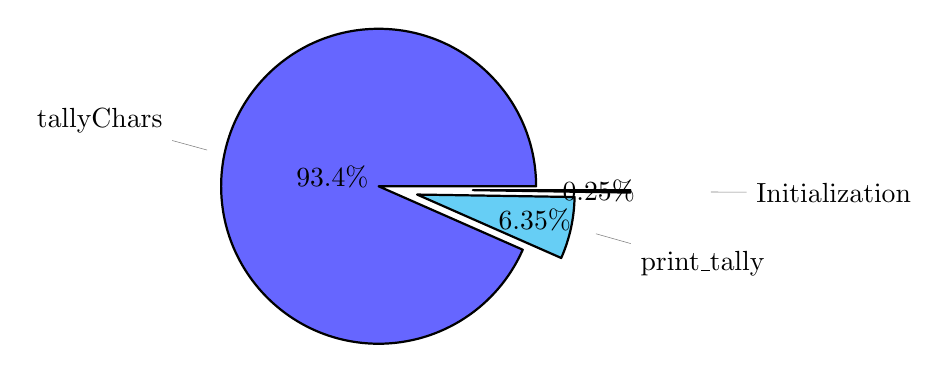
\begin{tikzpicture}
    \pie [rotate = 0, radius = 2, text = pin, explode = { 0.2, 0.3, 1}]
    {93.4/tallyChars, 6.35/print\_tally, 0.25/Initialization}
\end{tikzpicture}

% Cloud version test of chart
% \begin{tikzpicture}
%     \pie [cloud, text=legend, scale font, radius=3]
%     {93.4/tallyChars, 6.35/print\_tally, 0.25/Initialization}
% \end{tikzpicture}

\paragraph{Percent of execution time}
As seen on the pie chart, the tallyChars method is responsible for 93,4\% of the total runtime, this is a clear indication
of where we need to focus our optimization. The output to the console only takes up 6,35\% of the execution time. This means 
that optimization in this part of the program will have less infuence of the total runtime. However, the lowest amount of time 
is used in initialization, that only takes up 0,25\% of the total execution time. 

We can now try to plot the execution times in a boxplot. 
\begin{tikzpicture}
    \begin{axis}
      [
      ytick={1,2,3},
      yticklabels={Initialization, tallyChars, print\_tally},
      ]
      \addplot+[
      boxplot prepared={
        median=47,
        upper quartile=47,
        lower quartile=46,
        upper whisker=99,
        lower whisker=40
      },
      ] coordinates {};
      \addplot+[
      boxplot prepared={
        median=23,
        upper quartile=23,
        lower quartile=23,
        upper whisker=26,
        lower whisker=23
      },
      ] coordinates {};
      \addplot+[
      boxplot prepared={
          median=23,
          upper quartile=23,
          lower quartile=23,
          upper whisker=26,
          lower whisker=23
      },
      ] coordinates {};
    \end{axis}
  \end{tikzpicture}

\paragraph{Optimization}


code snippets of benchmark points
How did we make the benchmark method
What can be optimized

\section{Optimization}
What changes do we make to the program
Show snippets of changes

\section{Benchmark for Optimized}
show the results of the benchmark

\section{Benchmark Comparison}
Compare the original vs the optimized times
show tons of graphs and charts

\section{Conclusion}
Sum it up 
talk about most remarkable changes.


\end{document}